%author : berenice delcroix-oger

\documentclass[border=2pt]{standalone}
\usepackage{tikz}
\usetikzlibrary{positioning, fit, shapes, arrows, calc}

\pgfdeclarelayer{bg}    % declare background layer
\pgfsetlayers{bg,main}  % set the order of the layers (main is the standard layer)

\newcommand{\coula}{0785F2}
\newcommand{\coulb}{F29F05}
\newcommand{\coulc}{F21313}
\newcommand{\could}{E6F21F}

\definecolor{bleu}{HTML}{0000FF} 
\definecolor{vert}{HTML}{39B44B}
\definecolor{rouge}{HTML}{FF0000}


\definecolor{part1}{HTML}{\coula}
\definecolor{part2}{HTML}{\coulb}
\definecolor{part3}{HTML}{\coulc}
\definecolor{part4}{HTML}{\could}

\begin{document}
\begin{tikzpicture}
\node(12) {$F=$\begin{tikzpicture}[grow=up, inner sep=1pt,  outer sep=0pt, level distance=1cm, sibling distance=15pt, baseline=.9cm]
\node[draw, circle] {$1$}
   child[thick]{node[circle, fill=rouge, fill opacity=0.4, text opacity=1, anchor=center] {$5$}
          child{node[circle, fill=bleu, fill opacity=0.4, text opacity=1, anchor=center] {$3$}}
          child{node[circle, fill=vert, fill opacity=0.4, text opacity=1, anchor=center] {$4$}}     
   };
\end{tikzpicture}
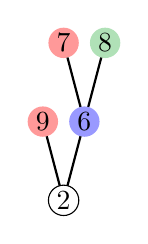
\begin{tikzpicture}[grow=up, inner sep=1pt, level distance=1cm, sibling distance=15pt,  outer sep=0pt, baseline=.9cm]
\node[draw, circle] {$2$}
   child[thick]{node[circle, fill=bleu, fill opacity=0.4, text opacity=1, anchor=center] {$6$}
          child{node[circle, fill=vert, fill opacity=0.4, text opacity=1, anchor=center] {$8$}}     
          child{node[circle, fill=rouge, fill opacity=0.4, text opacity=1, anchor=center] {$7$}}     
   }
   child[thick]{node[circle, fill=rouge, fill opacity=0.4, text opacity=1, anchor=center] {$9$}}
;
\end{tikzpicture}
};
\node[right=1cm of 12](3) {
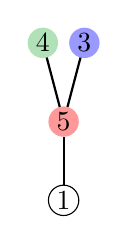
\begin{tikzpicture}[grow=up, inner sep=1pt,  outer sep=0pt, level distance=1cm, sibling distance=15pt, baseline=.9cm]
\node[draw, circle] {$1$}
   child[thick]{node[circle, fill=rouge, fill opacity=0.4, text opacity=1, anchor=center] {$5$}
          child{node[circle, fill=bleu, fill opacity=0.4, text opacity=1, anchor=center] {$3$}}
          child{node[circle, fill=vert, fill opacity=0.4, text opacity=1, anchor=center] {$4$}}     
   };
\end{tikzpicture}
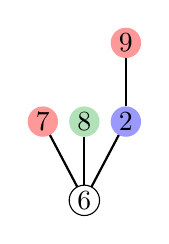
\begin{tikzpicture}[grow=up, inner sep=1pt, level distance=1cm, sibling distance=15pt,  outer sep=0pt, baseline=.9cm]
\node[draw, circle] {$6$}
   child[thick]{node[circle, fill=bleu, fill opacity=0.4, text opacity=1, anchor=center] {$2$}
          child{node[circle, fill=rouge, fill opacity=0.4, text opacity=1, anchor=center] {$9$}}}
          child[thick]{node[circle, fill=vert, fill opacity=0.4, text opacity=1, anchor=center] {$8$}}     
   child[thick]{node[circle, fill=rouge, fill opacity=0.4, text opacity=1, anchor=center] {$7$}}
;
\end{tikzpicture}
};
\draw[->] (12) edge[->] node[above] {(3)} (3);
\node[right=1cm of 3](45) {
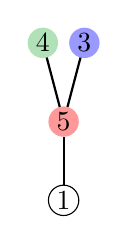
\begin{tikzpicture}[grow=up, inner sep=1pt,  outer sep=0pt, level distance=1cm, sibling distance=15pt, baseline=.9cm]
\node[draw, circle] {$1$}
   child[thick]{node[circle, fill=rouge, fill opacity=0.4, text opacity=1, anchor=center] {$5$}
          child{node[circle, fill=bleu, fill opacity=0.4, text opacity=1, anchor=center] {$3$}}
          child{node[circle, fill=vert, fill opacity=0.4, text opacity=1, anchor=center] {$4$}}     
   };
\end{tikzpicture}
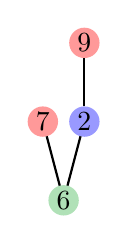
\begin{tikzpicture}[grow=up, inner sep=1pt, level distance=1cm, sibling distance=15pt,  outer sep=0pt, baseline=.9cm]
\node[circle, fill=vert, fill opacity=0.4, text opacity=1, anchor=center] {$6$}
   child[thick]{node[circle, fill=bleu, fill opacity=0.4, text opacity=1, anchor=center] {$2$}
          child{node[circle, fill=rouge, fill opacity=0.4, text opacity=1, anchor=center] {$9$}}}
   child[thick]{node[circle, fill=rouge, fill opacity=0.4, text opacity=1, anchor=center] {$7$}}
;
\end{tikzpicture}

\begin{tikzpicture}[grow=up, inner sep=1pt, level distance=1cm, sibling distance=20pt,  outer sep=0pt, baseline=.9cm]
\node[circle, fill=vert, fill opacity=0.4, text opacity=1, anchor=center] {$8$};
\end{tikzpicture}
};
\draw[->] (3) edge[->] node[above] {(4)(5)} (45);
\node[right=1cm of 45](6) {
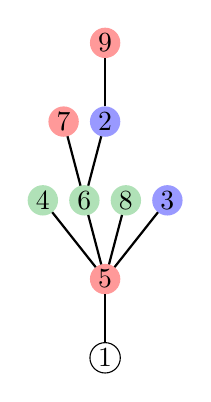
\begin{tikzpicture}[grow=up, inner sep=1pt,  outer sep=0pt, level distance=1cm, sibling distance=15pt, baseline=1.9cm]
\node[draw, circle] {$1$}
   child[thick]{node[circle, fill=rouge, fill opacity=0.4, text opacity=1, anchor=center] {$5$}
          child{node[circle, fill=bleu, fill opacity=0.4, text opacity=1, anchor=center] {$3$}}
          child{node[circle, fill=vert, fill opacity=0.4, text opacity=1, anchor=center] {$8$}}
          child{node[circle, fill=vert, fill opacity=0.4, text opacity=1, anchor=center] {$6$}
   child[thick]{node[circle, fill=bleu, fill opacity=0.4, text opacity=1, anchor=center] {$2$}
          child{node[circle, fill=rouge, fill opacity=0.4, text opacity=1, anchor=center] {$9$}}}
   child[thick]{node[circle, fill=rouge, fill opacity=0.4, text opacity=1, anchor=center] {$7$}}}
          child{node[circle, fill=vert, fill opacity=0.4, text opacity=1, anchor=center] {$4$}}     
   };
\end{tikzpicture} $=G$
};
\draw[->] (45) edge[->] node[above] {(6)} (6);
\end{tikzpicture}
\end{document}
